\documentclass{article}\usepackage[]{graphicx}\usepackage[]{xcolor}
% maxwidth is the original width if it is less than linewidth
% otherwise use linewidth (to make sure the graphics do not exceed the margin)
\makeatletter
\def\maxwidth{ %
  \ifdim\Gin@nat@width>\linewidth
    \linewidth
  \else
    \Gin@nat@width
  \fi
}
\makeatother

\definecolor{fgcolor}{rgb}{0.345, 0.345, 0.345}
\newcommand{\hlnum}[1]{\textcolor[rgb]{0.686,0.059,0.569}{#1}}%
\newcommand{\hlstr}[1]{\textcolor[rgb]{0.192,0.494,0.8}{#1}}%
\newcommand{\hlcom}[1]{\textcolor[rgb]{0.678,0.584,0.686}{\textit{#1}}}%
\newcommand{\hlopt}[1]{\textcolor[rgb]{0,0,0}{#1}}%
\newcommand{\hlstd}[1]{\textcolor[rgb]{0.345,0.345,0.345}{#1}}%
\newcommand{\hlkwa}[1]{\textcolor[rgb]{0.161,0.373,0.58}{\textbf{#1}}}%
\newcommand{\hlkwb}[1]{\textcolor[rgb]{0.69,0.353,0.396}{#1}}%
\newcommand{\hlkwc}[1]{\textcolor[rgb]{0.333,0.667,0.333}{#1}}%
\newcommand{\hlkwd}[1]{\textcolor[rgb]{0.737,0.353,0.396}{\textbf{#1}}}%
\let\hlipl\hlkwb

\usepackage{framed}
\makeatletter
\newenvironment{kframe}{%
 \def\at@end@of@kframe{}%
 \ifinner\ifhmode%
  \def\at@end@of@kframe{\end{minipage}}%
  \begin{minipage}{\columnwidth}%
 \fi\fi%
 \def\FrameCommand##1{\hskip\@totalleftmargin \hskip-\fboxsep
 \colorbox{shadecolor}{##1}\hskip-\fboxsep
     % There is no \\@totalrightmargin, so:
     \hskip-\linewidth \hskip-\@totalleftmargin \hskip\columnwidth}%
 \MakeFramed {\advance\hsize-\width
   \@totalleftmargin\z@ \linewidth\hsize
   \@setminipage}}%
 {\par\unskip\endMakeFramed%
 \at@end@of@kframe}
\makeatother

\definecolor{shadecolor}{rgb}{.97, .97, .97}
\definecolor{messagecolor}{rgb}{0, 0, 0}
\definecolor{warningcolor}{rgb}{1, 0, 1}
\definecolor{errorcolor}{rgb}{1, 0, 0}
\newenvironment{knitrout}{}{} % an empty environment to be redefined in TeX

\usepackage{alltt}
\usepackage[utf8]{inputenc}
\usepackage{amsfonts}
\usepackage{tgpagella}
\usepackage{graphicx} % Required for inserting images
\usepackage{polski}
\renewcommand*{\figurename}{Rysunek}
\usepackage{nicefrac, xfrac}
\usepackage[margin=1in]{geometry}
\usepackage{hyperref}
\usepackage{xcolor}
\usepackage{amssymb}
\usepackage[bottom]{footmisc}
\usepackage{float}
\IfFileExists{upquote.sty}{\usepackage{upquote}}{}
\begin{document}



\section{Wstęp}

\section{Odsetek naprawianych marek pojazdów}
%Odsetek naprawianych marek pojazdów.

Przeprowadzono analizę, aby sprawdzić jakich marek pojazdy najczęściej pojawiają się w warsztacie do naprawy. 



Można przedstawić procentowy udział marek pojazdów klientów salonu, zaczynając od najczęściej się pojawiającej:

\begin{verbatim}
1. Volkswagen: 13.36%
2. Opel: 8.97%
3. Ford: 8.4%
4. Skoda: 4.96%
5. Audi: 4.96%
6. Renault: 4.77%
7. Mercedes-Benz: 4.2%
8. SEAT: 4.01%
9. Fiat: 4.01%
10. Hyundai: 3.44%
11. Bajaj: 3.44%
12. Peugeot: 3.24%
13. BMW: 2.67%
14. Honda: 2.67%
15. Toyota: 2.67%
16. Hero: 2.29%
17. Nissan: 2.1%
18. Suzuki: 2.1%
19. Citroen: 1.91%
20. Kia: 1.91%
21. Yamaha: 1.72%
22. Dacia: 1.34%
23. Volvo: 1.34%
24. smart: 1.34%
25. Royal: 1.34%
26. Mazda: 0.76%
27. Porsche: 0.76%
28. Land: 0.76%
29. MINI: 0.57%
30. Jeep: 0.57%
31. Mitsubishi: 0.57%
32. KTM: 0.57%
33. Jaguar: 0.38%
34. Chevrolet: 0.38%
35. TVS: 0.38%
36. Lamborghini: 0.19%
37. Activa: 0.19%
38. RAM: 0.19%
39. Kawasaki: 0.19%
40. Subaru: 0.19%
41. Alfa: 0.19%
\end{verbatim}

Jak widać, najpopularniejsze są pojazdy marki Volkswagen. Pojazdy tej marki stanowią 13.36\% wszystkich. \\

Najmniej popularne są marki Activa, RAM, Kawasaki, Subaru, Alfa i Lamborghini. Każdą z nich reprezentowało 0.19\% pojazdów, które się pojawiły w warsztacie. \\

Ilość pojazdów, które były w warsztacie to \ensuremath{2.5940594\times 10^{-321}}. Było więcej samochodów niż motorów. Różnica między ilością typu pojazdu wynosiła \ensuremath{1.9108911\times 10^{-321}}, a samochodów było \ensuremath{2.2524752\times 10^{-321}}).

Sprawdzono także, jak prezentowałyby się rozkład marek, gdyby brano pod uwagę jedynie samochody



Można przedstawić ranking marek, zaczynając od najczęściej się pojawiającej:

\begin{verbatim}
1. Volkswagen: 15.38%
2. Opel: 10.33%
3. Ford: 9.67%
4. Skoda: 5.71%
5. Audi: 5.71%
6. Renault: 5.49%
7. Mercedes-Benz: 4.84%
8. SEAT: 4.62%
9. Fiat: 4.62%
10. Hyundai: 3.96%
11. Peugeot: 3.74%
12. BMW: 3.08%
13. Toyota: 3.08%
14. Nissan: 2.42%
15. Citroen: 2.2%
16. Kia: 2.2%
17. Dacia: 1.54%
18. smart: 1.54%
19. Volvo: 1.54%
20. Suzuki: 1.54%
21. Land: 0.88%
22. Mazda: 0.88%
23. Porsche: 0.88%
24. Jeep: 0.66%
25. Mitsubishi: 0.66%
26. MINI: 0.66%
27. Honda: 0.44%
28. Jaguar: 0.44%
29. Chevrolet: 0.44%
30. Alfa: 0.22%
31. RAM: 0.22%
32. Lamborghini: 0.22%
33. Subaru: 0.22%
\end{verbatim}

Wśród aut prym wiedzie Volkswagen, reprezentując  15.38\% naprawianych samochodów. \\

Najmniej było samochodów marek RAM, Lamborghini, Subaru i Alfa. Było ich 0.22\% dla każdej. \\

Pozostały do sprawdzenia motory.



Udział procentowy poszczególnych marek wśród nich prezentuje się następująco:

\begin{verbatim}
1. Bajaj: 26.09%
2. Hero: 17.39%
3. Honda: 17.39%
4. Yamaha: 13.04%
5. Royal: 10.14%
6. Suzuki: 5.8%
7. KTM: 4.35%
8. TVS: 2.9%
9. Kawasaki: 1.45%
10. Activa: 1.45%
\end{verbatim}

Wśród nich najczęściej naprawiano motory marki Bajaj. Pojazdy tej marki stanowią 26.09\% wszystkich. \\

Najmniej popularnymi motorami są z kolei modele marek Activa i Kawasaki. W warsztacie było zaledwie 1.45\% motorów każdej z wymienionych marek.

\section{Liczba naprawianych pojazdów w każdym miesiącu pracy warsztatu}

\begin{knitrout}
\definecolor{shadecolor}{rgb}{0.969, 0.969, 0.969}\color{fgcolor}\begin{figure}[H]

{\centering 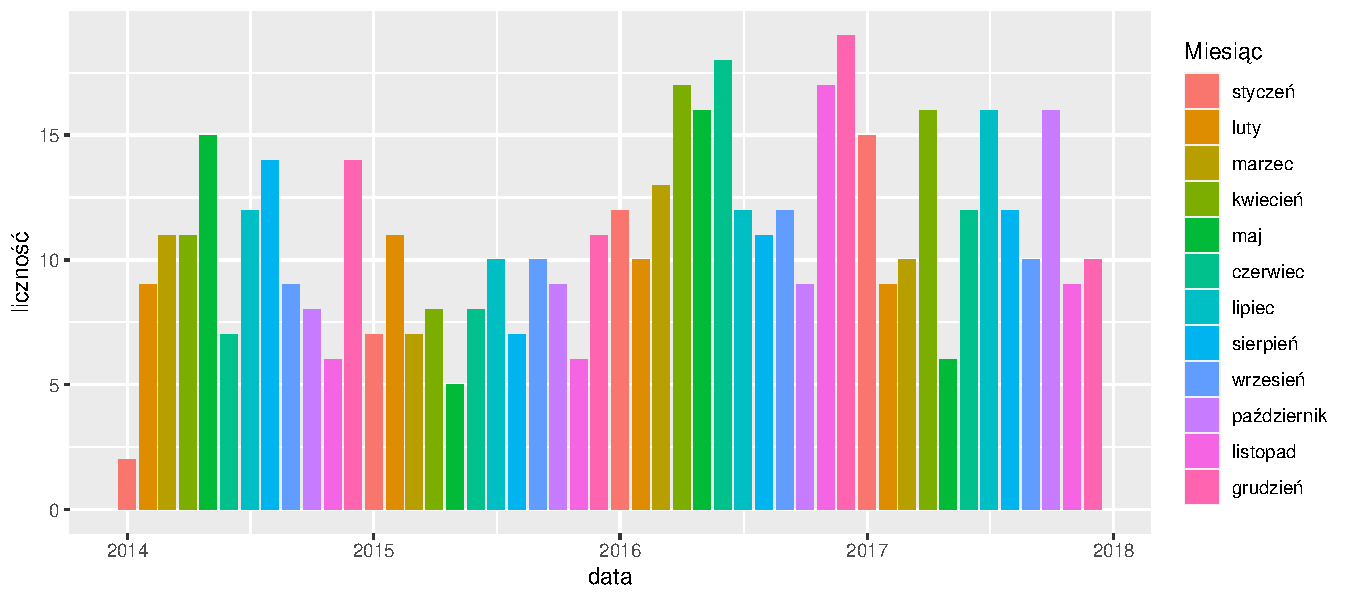
\includegraphics[width=\maxwidth]{figure/fig_naprawy_miesiecznie-1} 

}

\caption[Wykres liczba naprawianych pojazdów w każdym miesiącu pracy warsztatu]{Wykres liczba naprawianych pojazdów w każdym miesiącu pracy warsztatu}\label{fig:fig_naprawy_miesiecznie}
\end{figure}

\end{knitrout}

Wykres \ref{fig:fig_naprawy_miesiecznie} przedstawia liczbę naprawionych pojazdów w każdym miesiącu pracy warsztatu. Najwięcej pojazdów zostało naprawionych w miesiącach: 
grudzień 2016,
a było ich 19. Natomiast najmniej przeprowadzonych napraw było w miesiącach:
styczeń 2014,
było ich 2. Średnia liczba napraw miesięcznie wynosi 
10.917. 

\section{Tabela najlepszych okazji}

Zostanie teraz omówiona tabela najlepszych okazji, czyli pojazdów skupionych i sprzedanych, które przyniosły najwięcej zysku. Został uwzględniony także koszt naprawy pojazdu, gdy była ona potrzebna.





\begin{knitrout}
\definecolor{shadecolor}{rgb}{0.969, 0.969, 0.969}\color{fgcolor}\begin{kframe}
\begin{verbatim}
##     id_samochodu         marka       model   zysk
## 522          694   Lamborghini   Aventador 106792
## 353          455           BMW         640  96514
## 710          913         Aston Martin DB11  89268
## 578          761 Mercedes-Benz    A 45 AMG  76952
## 558          223 Mercedes-Benz     GLE 500  76776
\end{verbatim}
\end{kframe}
\end{knitrout}

Największy zysk ze sprzedaży pojazdu warsztat odniósł dla pojazdu o id 694. Jest nim Lamborghini o modelu Aventador. Warsztat zarobił on na nim około 106.79 tys. zł. 
Na drugim miejscu znajduje się BMW o modelu 640. Zysk z tego pojazdu wyniósł około 96.51 tys. zł, czyli o około 10.28 tys. zł mniej niż dla pojazdu znajdującego się na pierwszym miejscu, czyli różnica w cenie jest duża.
W trzeciej kolejności najwięcej zarobił pojazd Aston o modelu Martin DB11, na którym warsztat zarobił około 89.27 tys. zł. Jest to mniej od poprzedniego pojazdu o około 7.24 tys. zł, czyli różnica w cenie jest średniej wielkości. 
Ogólnie każdy pojazd znajdujący się w top 5 najlepszych okazji przyniósł zysk wielkości przynajmnej 80 tyś. zł.

\section{Profil klienta}

W następnej kolejności zostaną przeanalizawani klienci warsztatu. Zostaną sprawdzone liczności klientów ze względu na różne ich cechy.

\subsection{Płeć}

Pierwszą cechą wziętą pod uwagę jest płeć klienta. Zostanie sprawdzone, ile jest kobiet i mężczyzn wśród naszych klientów oraz jak duża jest różnica w licznościach tych grup.

\begin{knitrout}
\definecolor{shadecolor}{rgb}{0.969, 0.969, 0.969}\color{fgcolor}\begin{figure}[H]

{\centering 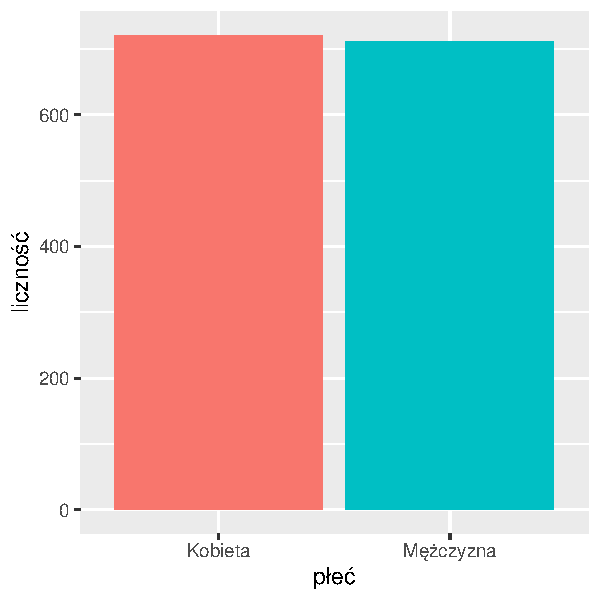
\includegraphics[width=\maxwidth]{figure/fig_plec-1} 

}

\caption[Wykres liczby klientów przy podziale ze względu na płeć]{Wykres liczby klientów przy podziale ze względu na płeć}\label{fig:fig_plec}
\end{figure}

\end{knitrout}

Na wykresie słupkowym \ref{fig:fig_plec} są zaprezentowane liczności klientów przy podziale ze względu na płeć. Więcej klientów warsztatu należy do grupy kobiet, jest ich 721. Grupa kobiet jest około 1.014
razy większa od grupy mężczyzn (jest ich 711), a zatem różnica jest nieduża.

\subsection{Wiek}

Zostanie również przeanalizowany rozkład wieku klientów warsztatu.





\begin{knitrout}
\definecolor{shadecolor}{rgb}{0.969, 0.969, 0.969}\color{fgcolor}\begin{figure}[H]

{\centering 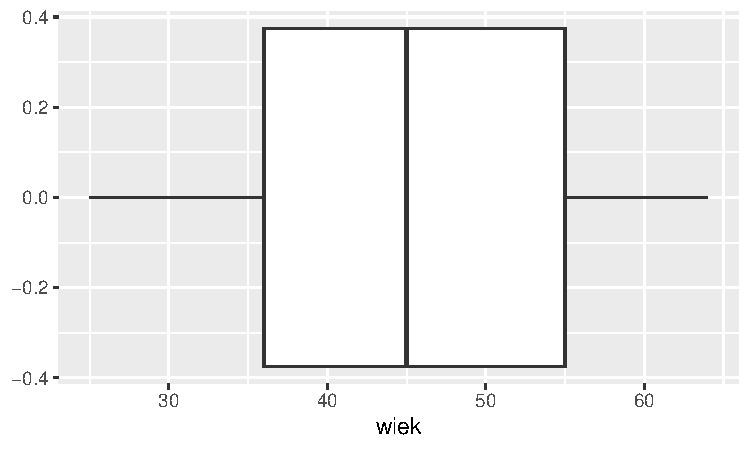
\includegraphics[width=\maxwidth]{figure/fig_wiek-1} 

}

\caption[Wykres pudełkowy wieku klientów]{Wykres pudełkowy wieku klientów}\label{fig:fig_wiek}
\end{figure}

\end{knitrout}

Rysunek \ref{fig:fig_wiek} przedstawia wykres pudełkowy wieku klientów warsztatu. Widać, że mediana wieku wynosi 45 lat, natomiast pierwszy kwartyl wynosi 36 lat, trzeci kwartyl natomiast 55 lat. Zatem połowa klientów warsztatu jest wieku między 36 lat a 55 lat.
Najmłodszy klient warsztatu ma 25 lat, natomiast najstarszy jest w wieku 64 lat.



\begin{table}[H]
\centering
\begin{tabular}{c|c} \hline
Miara & Wartość \\ \hline
Średnia & 45.4 \\ 
Odchylenie standardowe & 10.92 \\
Skośność & 0.02  \\ 
Kurtoza & 1.78 \\ \hline
\end{tabular}
\caption{Wybrane miary wieku klientów}
\label{tab_wiek}
\end{table}

Kilka miar, których nie da się odczytać z wykresu pudełkowego, zostało przedstawionych w tabeli \ref{tab_wiek}. Można zatem odczytać, że średnio klieci mają 45.4 lata, a odchylenie standardowe wieku wynosi 10.92 lata. Wartość współczynnika skośności jest bliska 0, a zatem rozkład wieku można uznać za symetryczny. Kurtoza przyjmuje wartość większą od 0, a zatem rozkład wieku jest leptokurtyczny, czyli jest bardziej wysmukły niż normalny.

\subsection{Miasto}
\begin{knitrout}
\definecolor{shadecolor}{rgb}{0.969, 0.969, 0.969}\color{fgcolor}\begin{kframe}
\begin{verbatim}
##   miejsce   miasto liczność
## 1       1  Wrocław      782
## 2       2     Łódź       24
## 3       3   Poznań       23
## 4       4 Szczecin       21
\end{verbatim}
\end{kframe}
\end{knitrout}

Najwięcej klientów warsztatu pochodzi z miasta Wrocław. Liczniść w nim wynosi 782 klientów. W następnej kolejności najwięcej klientów pochodzi z miasta Łódź, z czego liczność w nim wynosi 24 klientów, czyli jest ich 32.58 mniej niż klientów z miasta Wrocław. Na miejscu 3 jest miasto Poznań, mieszka w nim 23 klientów. Natomiast na ostatnim miejscu przedstawionym w tabeli jest miasto Szczecin, mieszka w nim 21 klientów.

\subsection{Karta lojalnościowa}

W tej części zostanie sprawdzone, ilu klientów posiada kartę lojalnościową. Klient zdobywa ją po skorzystaniu z usług warsztatu (naprawa, zakup lub sprzedaż pojazdu) przynajmniej trzy razy. Klient posiadający tę katrę może kupować samochody ze zniżką w wysokości 3\%.

\begin{knitrout}
\definecolor{shadecolor}{rgb}{0.969, 0.969, 0.969}\color{fgcolor}\begin{figure}[H]

{\centering 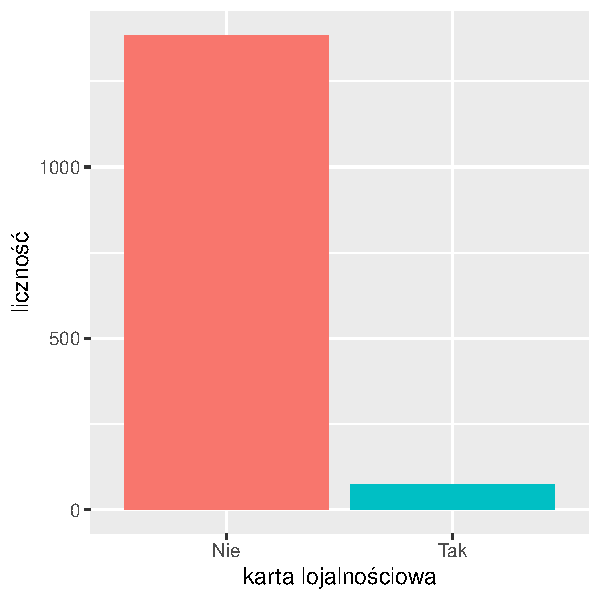
\includegraphics[width=\maxwidth]{figure/fig_karta-1} 

}

\caption[Wykres liczby klientów ze względu na posiadanie karty lojalnościowej]{Wykres liczby klientów ze względu na posiadanie karty lojalnościowej}\label{fig:fig_karta}
\end{figure}

\end{knitrout}

Bardzej liczną grupą są klienci, którzy nie posiadają karty lojalnoścowej, jest ich 1355 (95\% wszystkich klientów). W grupie klientów, którzy posiadają kartę lojalnoścową, jest 77 osób i stanowią oni 5\% klientów warsztatu.

\section{Jak wybrane cechy pojazdów wpływają na zysk warsztatu?}

W tym paragrafie zostaną opisane zależności między zyskiem ze sprzedaży pojazdów, skupionych i w razie potrzeby naprawionych przez warsztat, a cechami: rodzaj pojazdu, czy jest powypadkowy i pojemność silnika.

\subsection{Rodzaj pojazdu}

Pierwszą cechą braną pod uwagę jest rodzaj pojazdu, czyli czy jest to samochód czy motocykl.

\begin{knitrout}
\definecolor{shadecolor}{rgb}{0.969, 0.969, 0.969}\color{fgcolor}\begin{figure}[H]

{\centering 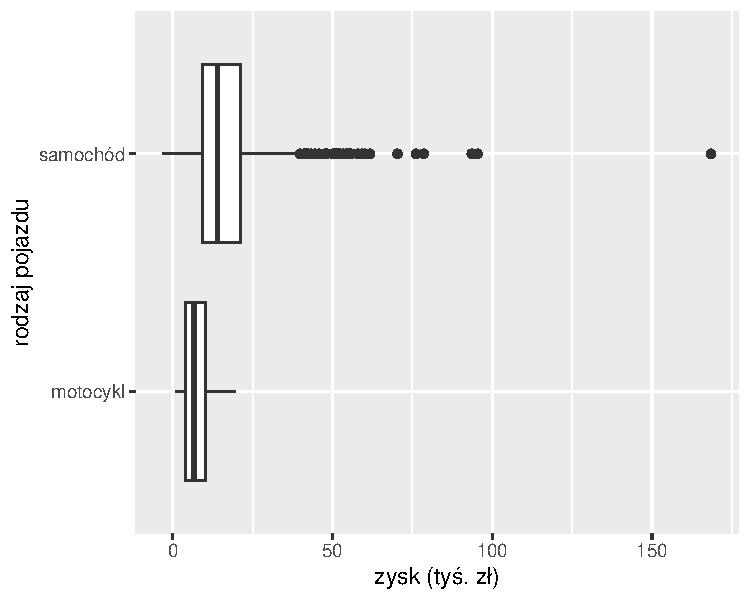
\includegraphics[width=\maxwidth]{figure/fig_typ-1} 

}

\caption[Wykresy pudełkowe zysku ze względu na rodzaj pojazdu]{Wykresy pudełkowe zysku ze względu na rodzaj pojazdu}\label{fig:fig_typ}
\end{figure}

\end{knitrout}

Na rysunku \ref{fig:fig_typ} przedstawione są dwa wykresy pudełkowe zysków, jeden dla samochodów, drugi dla motocykli. Większa mediana, wynosząca 14.384 tyś. zł, jest dla pojazdów typu samochód. W drugiej grupie wynosi ona 7.264 tyś. zł. 
Większy pierwszy kwartyl występuje w grupie typu samochód, wynosi on 9.458 tyś. zł, w porównaniu dla grupy typu motocykl jego wartość wynosi 4.5035 tyś. zł.
W przypadku kwartyla trzeciego większa wartość występuje w grupie typu samochód (wynosi 22.442 tyś. zł). W drugiej grupie wynosi on 10.926 tyś. zł.
Największy zysk przyniósł samochód, a wyniósł on 106.792 tyś. zł. 
Najmniejszy zysk natomiast przyniósł samochód i wyniósł on 0.3 tyś. zł. Zatem częściej większy zysk dla warsztatu przynosi sprzedaż pojazdów typu samochód. 

\subsection{Czy powypadkowy}

Następną badaną cechą jest to, czy pojazd jest powypadkowy.

\begin{knitrout}
\definecolor{shadecolor}{rgb}{0.969, 0.969, 0.969}\color{fgcolor}\begin{figure}[H]

{\centering 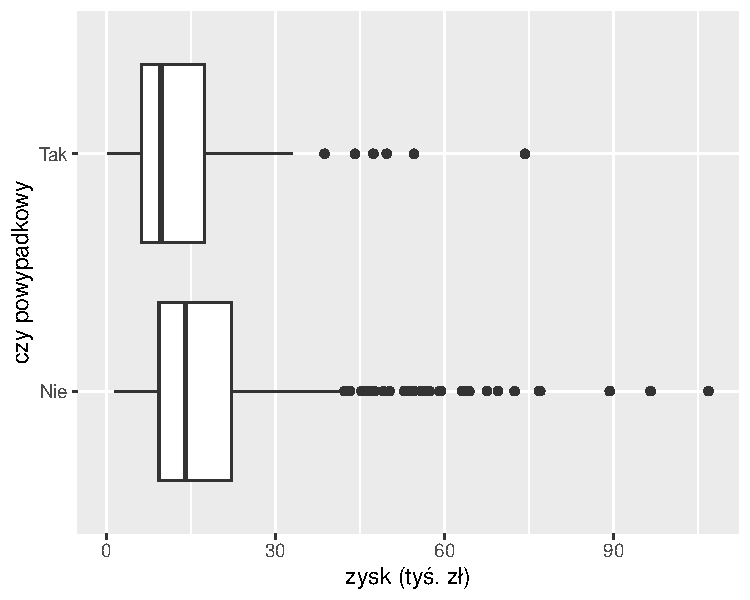
\includegraphics[width=\maxwidth]{figure/fig_wypadkowy-1} 

}

\caption[Wykresy pudełkowe zysku ze względu na to czy pojazd jest powypadkowy]{Wykresy pudełkowe zysku ze względu na to czy pojazd jest powypadkowy}\label{fig:fig_wypadkowy}
\end{figure}

\end{knitrout}

Na rysunku \ref{fig:fig_wypadkowy} przedstawione są dwa wykresy pudełkowe zysków dla pojazdów powypadkowych i niepowypadkowych. Większa mediana, wynosząca 14.048 tyś. zł, jest dla pojazdów niepowypadkowych. W drugiej grupie wynosi ona 9.679 tyś. zł. 
Większy pierwszy kwartyl występuje w grupie pojazdów niepowypadkowych, wynosi on 9.346 tyś. zł, w porównaniu dla grupy pojazdów powypadkowych jego wartość wynosi 6.316 tyś. zł.
Większa wartość trzeciego kwartylu występuje dla pojazdów niepowypadkowych i wynosi 22.2 tyś. zł. Dla pojazdów powypadkowych wynosi on 17.378 tyś. zł.
Największy zysk przyniósł pojazd z grupy niepowypadkowych i wyniósł on 106.792 tyś. zł. 
Najmniejszy zysk natomiast przyniósł pojazd z grupy powypadkowych i wyniósł on 0.3 tyś. zł. Zatem częściej większy zysk dla warsztatu przynosi sprzedaż pojazdów niepowypadkowych. 

\subsection{Pojemność silnika}

Ostatnią cechą braną pod uwagę jest pojemność silnika pojazdu.

\begin{knitrout}
\definecolor{shadecolor}{rgb}{0.969, 0.969, 0.969}\color{fgcolor}\begin{figure}[H]

{\centering 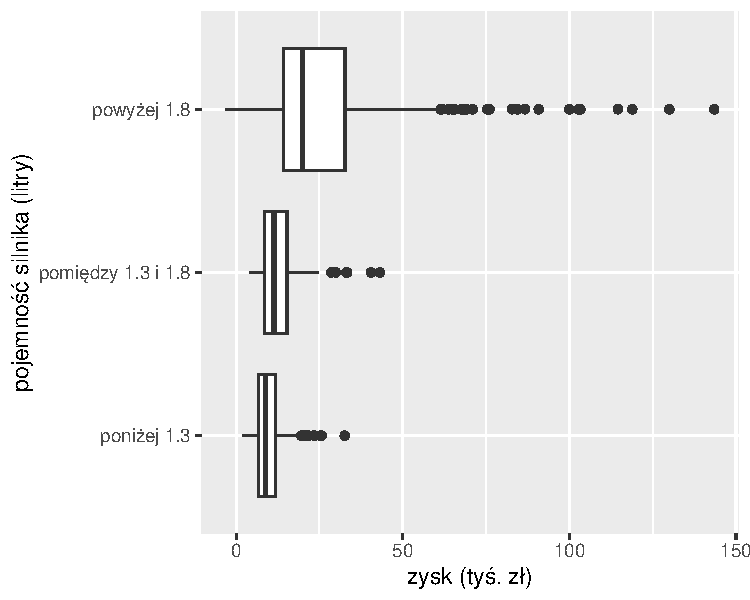
\includegraphics[width=\maxwidth]{figure/fig_pojemnosc-1} 

}

\caption[Wykresy pudełkowe zysku ze względu na pojemność silnika]{Wykresy pudełkowe zysku ze względu na pojemność silnika}\label{fig:fig_pojemnosc}
\end{figure}

\end{knitrout}

Na rysunku \ref{fig:fig_wypadkowy} przedstawione są wykresy pudełkowe zysków ze względu na pojemność silnika. Największa mediana, wynosząca 20.95 tyś. zł, jest dla pojazdów o pojemności silnika powyżej 1.8 litra. Natomiast najmniej ona wynosi 8.4 tyś. zł w grupie pojazdów o pojemności poniżej 1.3 litra. 
Największy pierwszy kwartyl występuje w grupie pojazdów o pojemności powyżej 1.8 litra, wynosi on 14.30375 tyś. zł, w porównaniu z pojazdami o pojemności poniżej 1.3 litra, dla których jego wartość jest najmniejsza i wynosi 6.124 tyś. zł.
Największa wartość trzeciego kwartylu występuje dla pojazdów o pojemności powyżej 1.8 litra i wynosi 29.7855 tyś. zł. Dla pojazdów poniżej 1.3 litra wynosi on 12 tyś. zł i jest to najmnijesza wartość w tych grupach.
Największy zysk przyniósł pojazd o pojemności silnika powyżej 1.8 litra i wyniósł on 106.792 tyś. zł. 
Najmniejszy zysk natomiast przyniósł pojazd z pojemnością silnika poniżej 1.3 litra i wyniósł on 0.3 tyś. zł. Zatem przeważnie największy zysk dla warsztatu przynosi sprzedaż pojazdów o pojemności silnika powyżej 1.8 litra. Najczęściej najmniejszy zysk przynosi sprzedaż pojazdów z pojemnością silnika poniżej 1.3 litra.

\section{Kim są najlepszy mechanik i sprzedawca w warsztacie?}

Przez czas działania warsztatu „Pimp My Wheels” osoba zarządzająca warsztatem nie była skłonna do dawania podwyżek, jednak postanowiła zlecić informatykowi by przeanalizował bazę danych i znalazł pracowników, którzy zasługują na większe wynagrodzenie. \\

Warsztatowi zależy na tym by sprzedawca zarobił dla firmy dużą kwotę (Może to osiągnąć sprzedając bardzo dużo pojazdów albo sprzedając wartościowe pojazdy), ale także by był charyzmatyczny i był w stanie przekonać wiele osób do zakupu. Rozważone wobec tego zostanie to który obecnie pracujący sprzedawca przekonał klientów do kupna największej liczby pojazdów, a który odpowiada za najwięcej środków pochodzących ze sprzedaży. \\


Tabela, w której są dane o sprzedawcach  pracujących w dowolnym momencie w warsztacie wygląda następująco:

\begin{knitrout}
\definecolor{shadecolor}{rgb}{0.969, 0.969, 0.969}\color{fgcolor}\begin{kframe}
\begin{verbatim}
##           sprzedawca     suma ile_sprzedanych płaca id_pracownika status
## 1     Stefania Berus 10107195             187  45.8             7      1
## 2 Liudmyla Dąbrowska 10802398             182  45.7             2      0
## 3         Paweł Kaza 11765080             192  53.2             3      1
## 4    Erwin Pudłowski 12078153             187  48.4             6      1
\end{verbatim}
\end{kframe}
\end{knitrout}

Jeżeli pracownik odszedł z warsztatu, to nielogicznym jest, by rozważać danie mu podwyżki.

Po usunięciu pracowników, którzy już nie pracują otrzymujemy taką tabelę:

\begin{knitrout}
\definecolor{shadecolor}{rgb}{0.969, 0.969, 0.969}\color{fgcolor}\begin{kframe}
\begin{verbatim}
##        sprzedawca     suma ile_sprzedanych płaca id_pracownika status
## 1  Stefania Berus 10107195             187  45.8             7      1
## 2      Paweł Kaza 11765080             192  53.2             3      1
## 3 Erwin Pudłowski 12078153             187  48.4             6      1
\end{verbatim}
\end{kframe}
\end{knitrout}

Osoba, która sprzedała pojazdy łącznie warte największą kwotę to Erwin Pudłowski. Zostały one zakupione przez klientów za 12078153.28 zł, co stanowi 107.95\% średniej sumy całej kwoty, którą wynegocjował z klientami sprzedawca przez cały okres pracy. Zarabiana przez tego pracownika kwota za godzinę pracy (48.40 zł) stanowi 100.26\% średniej płacy sprzedawcy (48.27 zł). Różnica procentowa wynosi 7.70\%, czyli warsztat zdecydowanie powinien rozważyć podwyżkę dla tego pracownika, by lepiej wyróżnić jego wpływ na dochody firmy. \\

Pracownik, który sprzedał najwięcej pojazdów to Paweł Kaza. Ten sprzedawca namówił klientów do kupna 192 pojazdów, co stanowi 102.67\% średnich sprzedaży przypadających na pracownika. Patrząc na zarobki pracownika można zauważyć, że zarabia on za godzinę pracy (53.20 zł), czyli 110.20\% średniej płacy sprzedawcy (48.27 zł). Różnica między tymi dwoma wartościami wynosi 7.53\% na korzyść pracownika, czyli zwiększenie stawki tego sprzedawcy nie jest niezbędne, lecz może go zmotywować. 

\begin{knitrout}
\definecolor{shadecolor}{rgb}{0.969, 0.969, 0.969}\color{fgcolor}\begin{kframe}
\begin{verbatim}
##               mechanik   suma ile_napraw płaca id_pracownika status
## 1        Agata Fangrat 112029        249  49.3             9      1
## 2       Paweł Suravets 157547        275  52.4             4      0
## 3 Ryszard Rzeszotarski 177657        251  59.6             8      1
\end{verbatim}
\end{kframe}
\end{knitrout}


Tutaj również należy usunąć z tabeli mechaników, którzy już nie pracują w warsztacie. \\

Pozostali następujący pracownicy:

\begin{knitrout}
\definecolor{shadecolor}{rgb}{0.969, 0.969, 0.969}\color{fgcolor}\begin{kframe}
\begin{verbatim}
##               mechanik   suma ile_napraw płaca id_pracownika status
## 1        Agata Fangrat 112029        249  49.3             9      1
## 2 Ryszard Rzeszotarski 177657        251  59.6             8      1
\end{verbatim}
\end{kframe}
\end{knitrout}

Mechanik, który wykonał w firmie naprawy, za które klienci (po odliczeniu kosztu części) zapłacili najwięcej to Ryszard Rzeszotarski i jest to kwota 177657.00 zł, co stanowi 119.17\% średniego zysku z napraw na mechanika. Pracownik zarabia kwotę 59.60 zł za godzinę pracy, co stanowi 110.85 \% średniej płacy mechanika (53.77 zł). Różnica między tymi wartościami to 8.32\%, wobec czego dobrze by było, gdyby firma zauważyła świetne wyniki tego pracownika i jego pozytywny wpływ na finanse warsztatu. \\

Pracownik, który dokonał największej liczby napraw to znów Ryszard Rzeszotarski. . Liczba napraw dokonana przez niego wynosi 251, co stanowi 97.29\% średniej ilości napraw na mechanika. Jej zarobki wynoszą 59.60 zł na godzinę, co stanowi 110.85 \% średniej płacy mechanika (53.77 zł). Różnica między tymi dwoma wartościami wynosi 13.56\% na korzyść pracownika, chociaż zwiększenie stawki może pozytywnie wpłynąć na efekty jego pracy.

\section{Analiza bilansu}

\subsection{Analiza wydatków na zakup pojazdów}

Sprawdziliśmy, jak wyglądają miesięczne wydatki na zakup pojazdów, które w razie potrzeby warsztat naprawia, a następnie sprzedaje.

\begin{knitrout}
\definecolor{shadecolor}{rgb}{0.969, 0.969, 0.969}\color{fgcolor}\begin{figure}[H]

{\centering 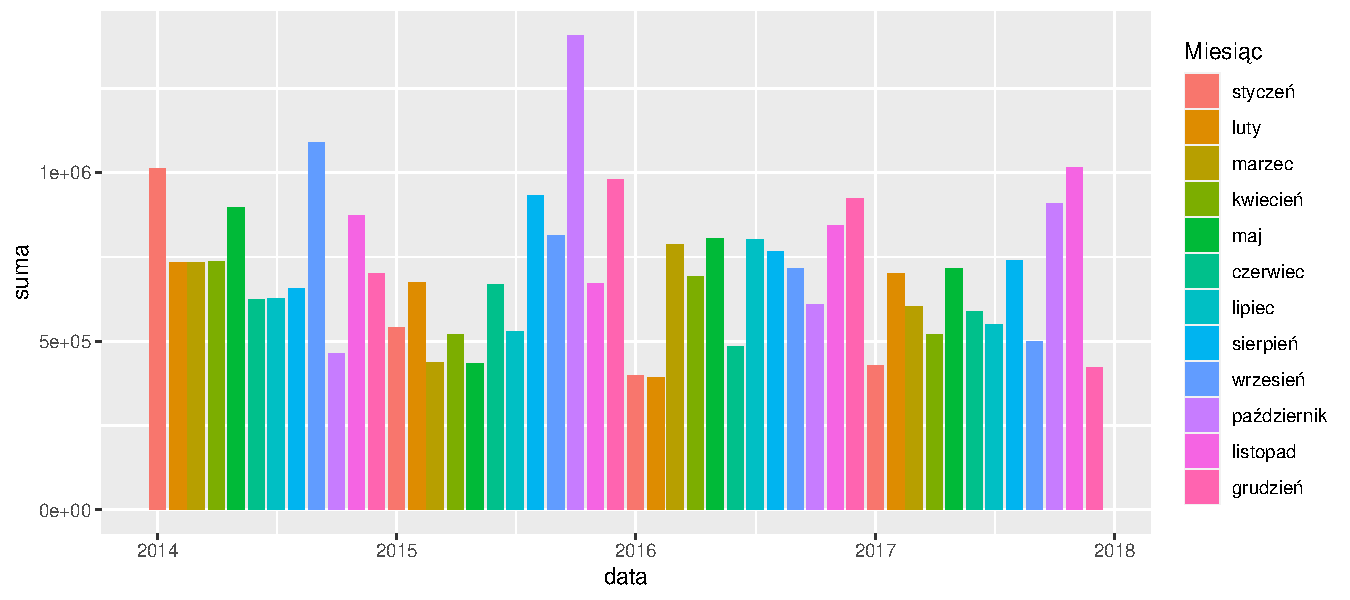
\includegraphics[width=\maxwidth]{figure/fig_zakup_pojazdu-1} 

}

\caption[Miesięczne wydatki na zakup pojazdów]{Miesięczne wydatki na zakup pojazdów}\label{fig:fig_zakup_pojazdu}
\end{figure}

\end{knitrout}

Wykres \ref{fig:fig_zakup_pojazdu} przedstawia miesięczne wydatki na zakup pojazdów. 
Największe wydatki warsztat miał w miesiącu maj 2017. Były one w wysokości 1158 tyś. zł. 
Wydatki wielkości 1128.5 tyś. zł były drugimi najwyższymi i były 1.03 razy mniejsze od tych największych. Wystąpiły one w miesiącu styczeń 2014.
Najmniejsze wydatki warsztat zaobserwował w miesiącu sierpień 2017 i wyniosły one 355.1 tyś. zł. 
Drugie co do wielkości najniższe wydatki na zakup pojazdów wystąpiły miesiącu grudzień 2016, a wyniosły one 371.6 tyś. zł.
W każdym miesiącu działania warsztatu wydatki na zakup pojazdów wyniosły przynajmnej 400 tyś. zł.

\subsection{Analiza wydatków na zakup części}

Następnie zostało sprawdzone, jak wyglądają miesięczne wydatki na zakup części potrzebnych do napraw pojazdów.

\begin{knitrout}
\definecolor{shadecolor}{rgb}{0.969, 0.969, 0.969}\color{fgcolor}\begin{figure}[H]

{\centering 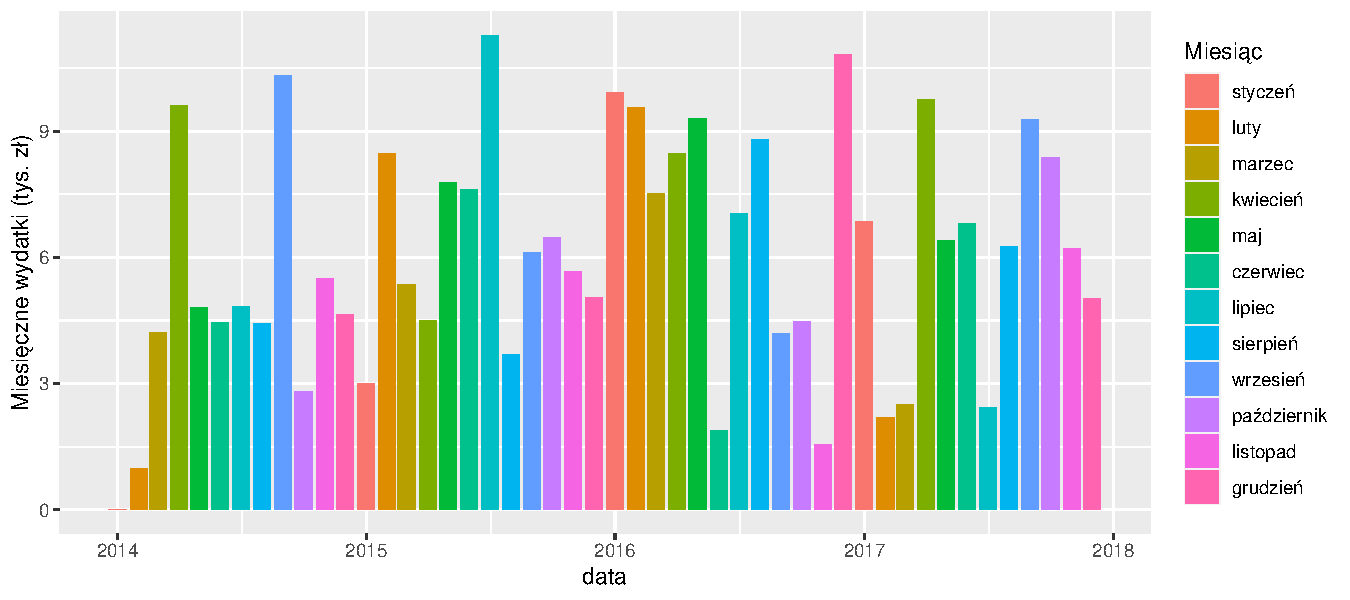
\includegraphics[width=\maxwidth]{figure/fig_zakup_czesci-1} 

}

\caption[Miesięczne wydatki na zakup części]{Miesięczne wydatki na zakup części}\label{fig:fig_zakup_czesci}
\end{figure}

\end{knitrout}

Wykres \ref{fig:fig_zakup_czesci} przedstawia miesięczne wydatki na zakup części do naprawy pojazdów.
Największe wydatki warsztat miał w miesiącu styczeń 2016 i wyniosły one 18.35 tyś. zł. 
Drugie najwyższye wydatkami były wielkości 17.6 tyś. zł i były 1.04 razy mniejsze od tych największych. Wystąpiły one w miesiącu lipiec 2014.
Najmniejsze wydatki na części zostały odnotowane w miesiącu styczeń 2014 i wyniosły 0.97 tyś. zł. 
Drugie najmniejsze wydatki wyniosły 1.09 tyś. zł. Wystąpił on w miesiącu styczeń 2015.
Ogólnie w każdym miesiącu działania warsztatu wydatki na zakup części wyniosły przynajmnej 1 tyś. zł.

\subsection{Analiza przychodów z usług warsztatu}

Chcielibyśmy sprawdzić, jak wyglądają miesięczne przychody (lub straty) wynikające z prowadzenia warsztatu. Przez przychód za pojedyńczą usługę uważamy różnicę ceny, którą zapłacił klient i kwoty zapłaconej za części. Przeanaliowane zostaną przychody z uwzględnieniem kosztu własnych napraw oraz bez nich.

\begin{knitrout}
\definecolor{shadecolor}{rgb}{0.969, 0.969, 0.969}\color{fgcolor}\begin{figure}[H]

{\centering 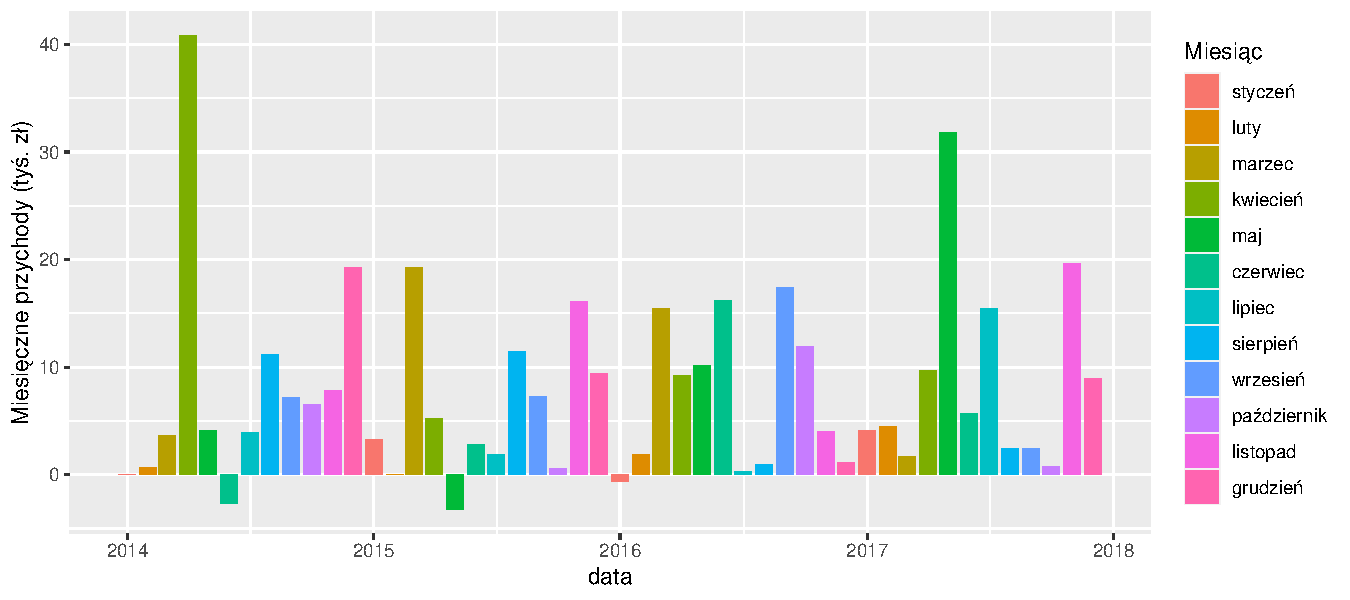
\includegraphics[width=\maxwidth]{figure/fig_uslugi-1} 

}

\caption[Miesięczny przychód wynikający z prowadzenia warsztatu z wliczonymi kosztami napraw własnych]{Miesięczny przychód wynikający z prowadzenia warsztatu z wliczonymi kosztami napraw własnych}\label{fig:fig_uslugi}
\end{figure}

\end{knitrout}

Na wykresie \ref{fig:fig_uslugi} przedstawiony jest miesięczny przychód wynikający z prowadzenia warsztatu. Zostały na nim uwzględnione koszty napraw własnych. 
Największy przychód był zaobserwowany w miesiącu styczeń 2016 i wyniósł on wtedy 45.44 tyś. zł.
Następny co do wielkości przychód wystąpił w miesiącu grudzień 2017, wyniósł on 22.8 tyś. zł. Jest on 1.99 razy mniejszy niż najwyższy przychód.
Najmniejszy przychód warsztat odnotował w miesiącu sierpień 2014, który wyniósł -1.32 tyś. zł. 
Drugi najmniejszy przychód wyniósł -0.56 tyś. zł i wystąpił w miesiącu kwiecień 2014.

\begin{knitrout}
\definecolor{shadecolor}{rgb}{0.969, 0.969, 0.969}\color{fgcolor}\begin{figure}[H]

{\centering 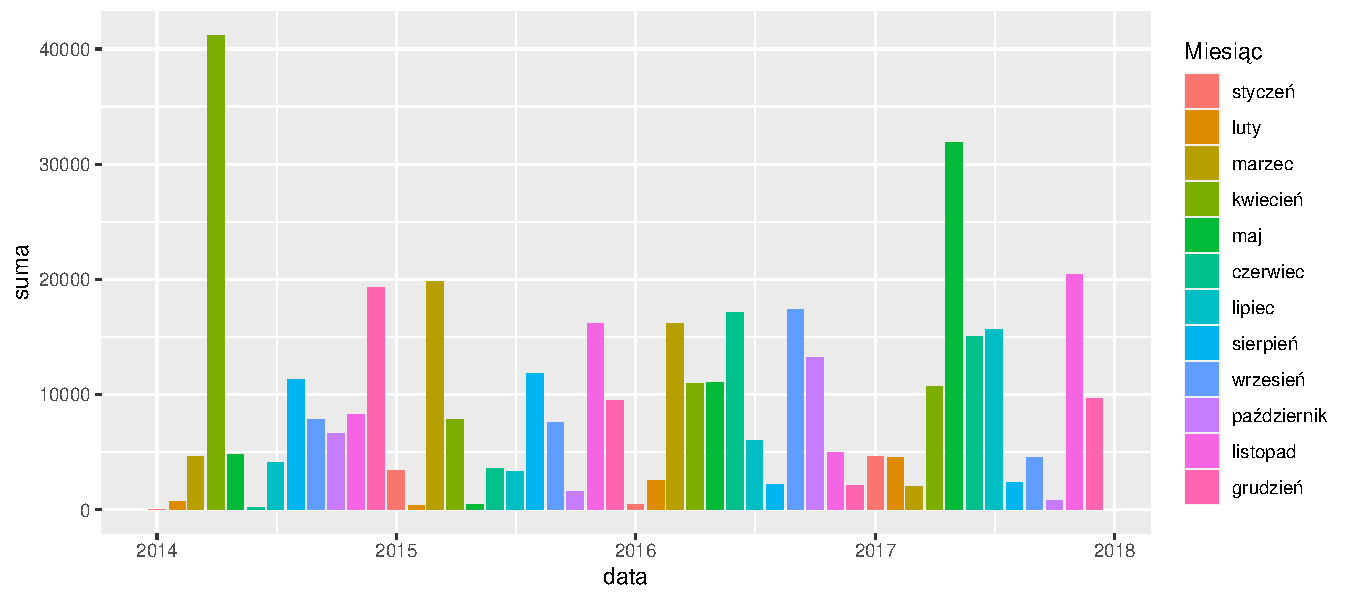
\includegraphics[width=\maxwidth]{figure/fig_uslugi2-1} 

}

\caption[Miesięczny przychód wynikający z prowadzenia warsztatu bez wliczonych kosztów napraw własnych]{Miesięczny przychód wynikający z prowadzenia warsztatu bez wliczonych kosztów napraw własnych}\label{fig:fig_uslugi2}
\end{figure}

\end{knitrout}

Na wykresie \ref{fig:fig_uslugi2} przedstawiony jest miesięczny przychód wynikający z prowadzenia warsztatu, ale tym razem bez uwzględnienia kosztów własnych. 
Największy przychód warsztat zaobserwował w miesiącu styczeń 2016, który wyniósł 45.44 tyś. zł.
Drugi zaś co do wielkości przychód wsytąpił w miesiącu marzec 2017, wyniósł on 27.25 tyś. zł, czyli jest 1.67 razy mniejszy niż ten najwyższy zaobserwowany.
Najmniejszy przychód został odnotowany w miesiącu styczeń 2015 i wyniósł 0.73 tyś. zł. 
Drugi najmniejszy przychód wyniósł 1.01 tyś. zł. Wystąpił on w miesiącu listopad 2014.

\subsection{Koszty wypłat dla pracowników}

Zostanie sprawdzone, jakie miesięczne koszty ponosi warsztat na wypłaty pensji dla pracowników.

%Zakładamy, że płaca w miesiącu to 160*płaca (przy zatrudnieniu/zwolnieniu pracownika patrze ile dni w miesiacu pracownik pracowal i robie ulamek, np. jak zatrudnili go 3 marca to dostaje round(płaca*160*29/31,2)) i podobnie ostatni to by byl round(płaca*160*3/31,2), wypłacamy pieniądze 1 dnia kolejnego miesiąca (np za styczeń wypłacamy 1 lutego)

\begin{knitrout}
\definecolor{shadecolor}{rgb}{0.969, 0.969, 0.969}\color{fgcolor}\begin{figure}[H]

{\centering 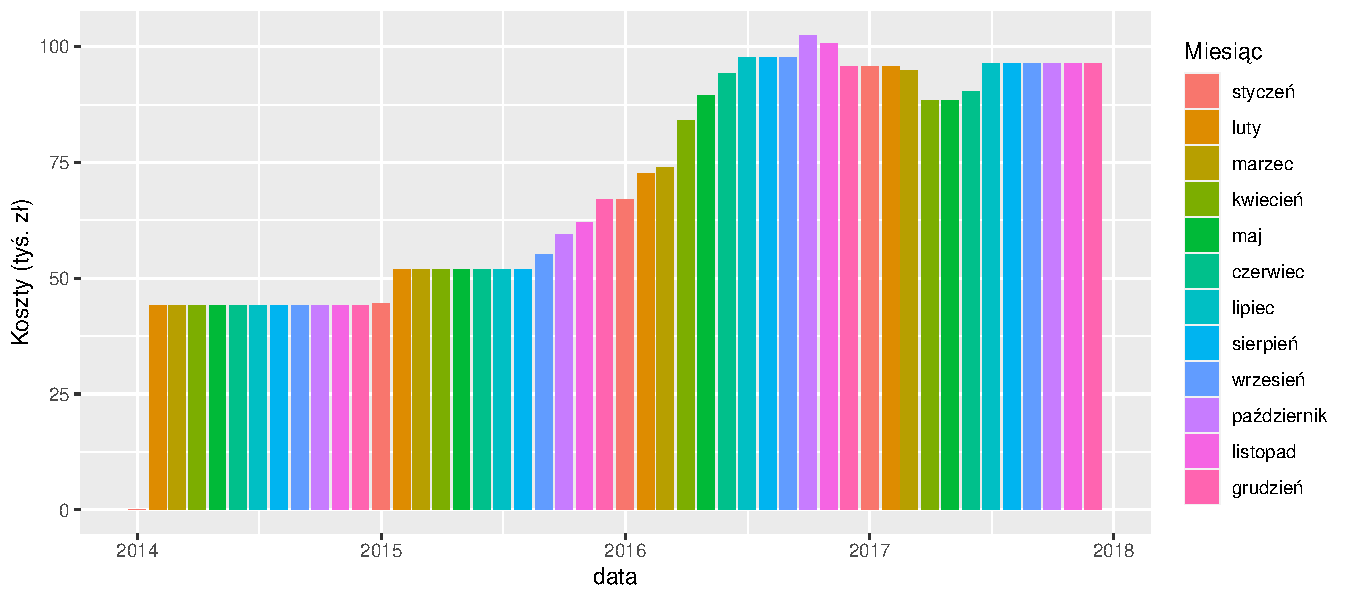
\includegraphics[width=\maxwidth]{figure/fig_pracownicy-1} 

}

\caption[Miesięczne koszty wynikające z wypłacania pensji pracownikom]{Miesięczne koszty wynikające z wypłacania pensji pracownikom}\label{fig:fig_pracownicy}
\end{figure}

\end{knitrout}

Wykres \ref{fig:fig_pracownicy} przedstawia miesięczne koszty wypłat pensji pracowników. Największy koszt warsztat odnotował w miesiącu listopad 2017 i wyniósł on 88.32 tyś. zł. 
Natomiast najmniejsze koszty wystąpiły w miesiącu styczeń 2014. Wyniosły one 0 zł. Wynika to z tego, że jest to pierwszy miesiąc działania warsztatu, a pensje wypłacamy pracownikom pierwszego dnia następnego miesiąca.

\subsection{Wpływy ze sprzedaży pojazdów}

Następnie zostaną sprawdzone miesięczne wpływy finansowe ze sprzedaży pojazdów, które zostały zakupione i w razie potrzeby naprawione przez warsztat. Pojazdy są sprzedawane na dwa sposoby: klient może zapłacić całą kwotę na raz lub spłacać w ratach. {\color{red}Jeśli klient zdecyduje się na pierwszą opcję, to przysługuje mu zniżka w wysokości (???).} {\color{red}Opisać: Jak są wpłaty to robimy dla wszystkich oprócz ostatniej floor z dzielenia, a ostatnia to cena zakupu - te raty co juz splacono}

\begin{knitrout}
\definecolor{shadecolor}{rgb}{0.969, 0.969, 0.969}\color{fgcolor}\begin{figure}[H]

{\centering 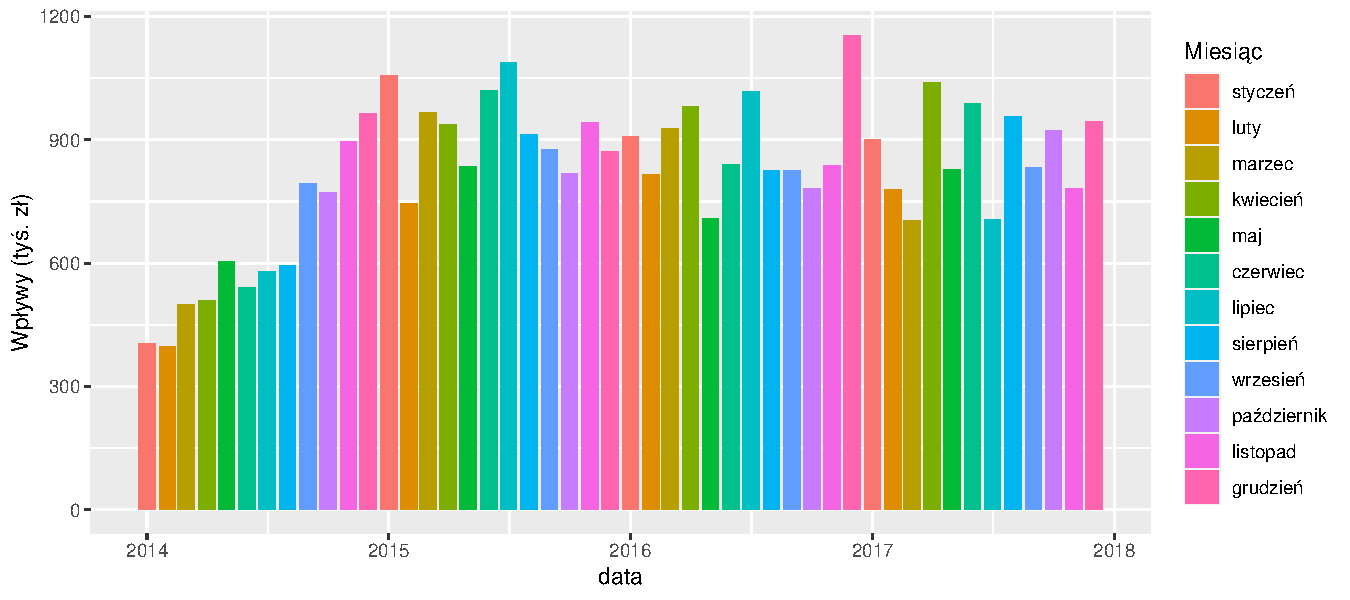
\includegraphics[width=\maxwidth]{figure/fig_samochody_wplywy-1} 

}

\caption[Miesięczne wpływy finansowe ze sprzedaży pojazdów]{Miesięczne wpływy finansowe ze sprzedaży pojazdów}\label{fig:fig_samochody_wplywy}
\end{figure}

\end{knitrout}

Na wykresie \ref{fig:fig_samochody_wplywy} przedstawione są wpływy finansowe ze sprzedaży pojazdów. 
Największe miesięczne wpływy warsztatu ze sprzedaży pojazdów wynosiły 1.21 mln. zł. Wystąpiły one w miesiącu luty 2015. 
Drugie co do wielkości wpływy (w wysokości 1.19 mln. zł) zostały odnotowane w miesiącu maj 2015. Są one 1.01 razy mniejsze niż te największe zaobserwowane.
Najmniejsze miesięczne wpływy wyniosły 0.28 mln. zł, a wystąpiły one w miesiącu luty 2014.
Kolejnymi najmniejszymi są wpływy z miesiącu marzec 2014. Są one wysokości 0.47 mln. zł.


\subsection{Bilans miesięczny}

Teraz zostanie sprawdzoby miesięczny bilans warsztatu. Zostaną sprawdzone miesięczne przychody warsztaty przez cały okres jego działania oraz comiesięczny stan środków finansowych firmy, gdyby warsztat zaczynał bez posiadania żadnych średków pienięznych.

\begin{knitrout}
\definecolor{shadecolor}{rgb}{0.969, 0.969, 0.969}\color{fgcolor}\begin{figure}[H]

{\centering 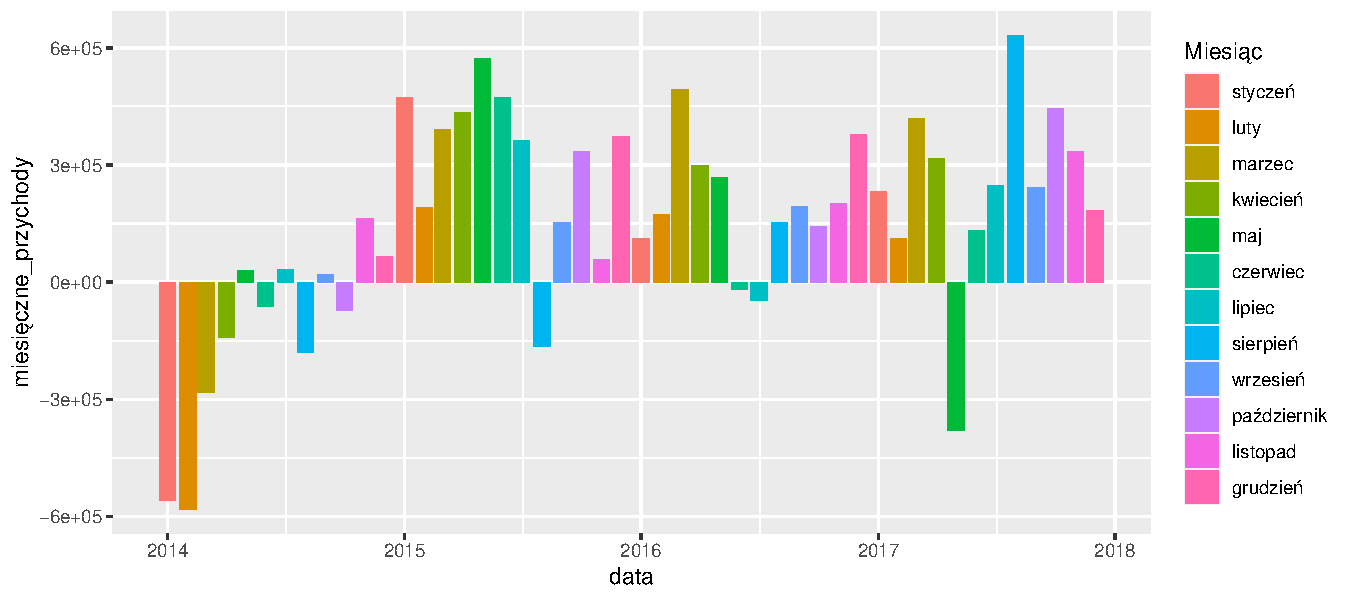
\includegraphics[width=\maxwidth]{figure/fig_bilans-1} 

}

\caption[Miesięczne przychody warsztatu]{Miesięczne przychody warsztatu}\label{fig:fig_bilans}
\end{figure}

\end{knitrout}

%złączenie: na miesiąc = naprawy(te z minusami, bo mają razem części) + sprzedaż pojazdu -zakup pojazdu - wypłaty (czy ja coś pominęłam?)

Wykres \ref{fig:fig_bilans} przedstawia miesięczne przychody firmy od początku jej działalności. 
Najwięcej warsztat zarobił (632.63 tyś. zł) w miesiącu sierpień 2017.
Natomiast najmniej w miesiącu luty 2014. Zyski wyniosły wtedy -583.32 tyś. zł. Przez pierwsze 4 miesięcy pracy warsztat nie przynosił żadnych zysków.

\begin{knitrout}
\definecolor{shadecolor}{rgb}{0.969, 0.969, 0.969}\color{fgcolor}\begin{figure}[H]

{\centering 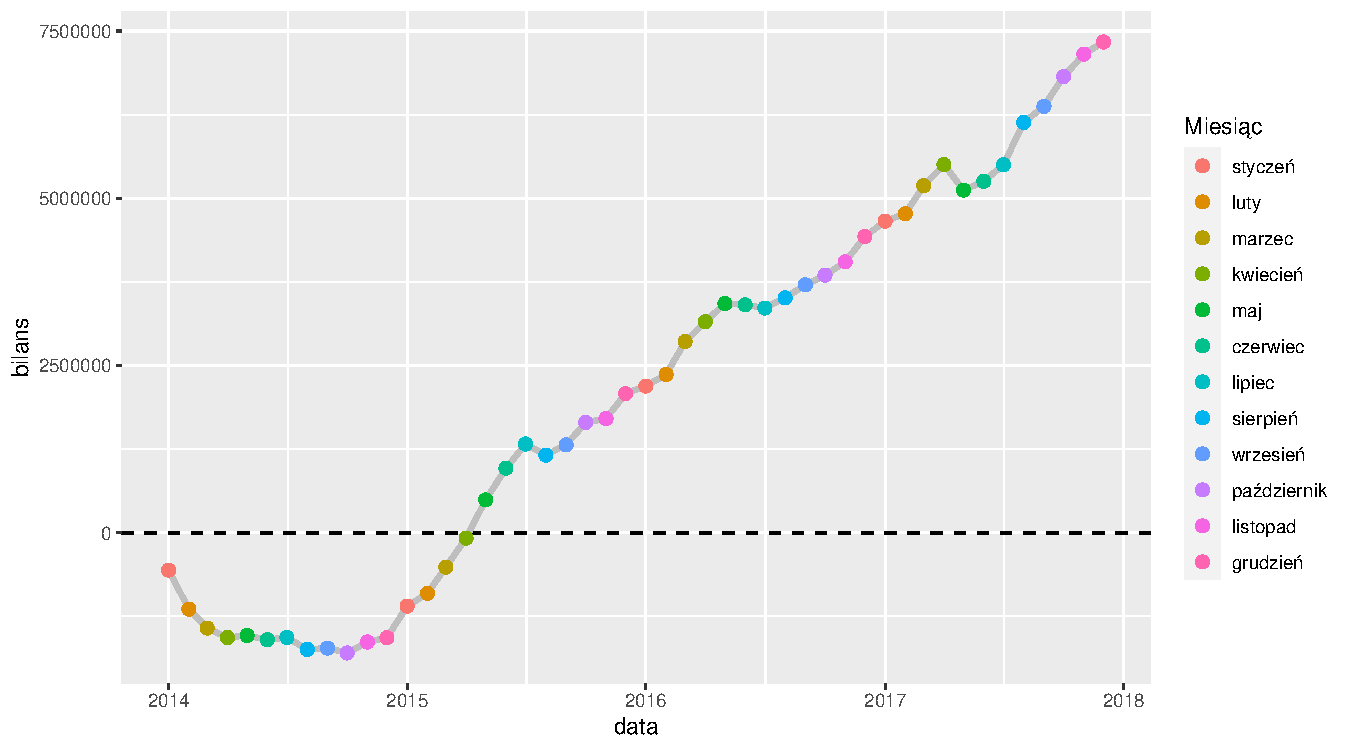
\includegraphics[width=\maxwidth]{figure/fig_bilans_suma-1} 

}

\caption[Miesięczny stan finansowy warsztatu, gdyby zaczynał działalność bez żadnych środków pieniężnych]{Miesięczny stan finansowy warsztatu, gdyby zaczynał działalność bez żadnych środków pieniężnych}\label{fig:fig_bilans_suma}
\end{figure}

\end{knitrout}

Wykres \ref{fig:fig_bilans_suma} przedstawia miesięczny stan finansowy warsztatu, gdyby zaczynał działalność bez środków pieniężnych. W pierwszym miesiącu działalności stan finansowy wyniósł -0.56 mln. zł, natomiast aktualnie wynosi on 7.34 mln. zł. Przez pierwsze 16 miesięcy pracy warsztatu jego stan finansowy był ujemny.
Największą ilością pieniędzy warsztat operował w miesiącu grudzień 2017, było to 7.34 mln. zł.
Natomiast najmniejszą w miesiącu październik 2014, a było to -1.8 mln. zł.

\section{Podsumowanie}





\end{document}
